\documentclass{article}

\usepackage[top=2.5cm, bottom=2.5cm, left=2cm, right=2cm]{geometry}
\usepackage{fancyhdr}
\lhead{\bsc{Projet Algorithmique Numerique}}
\rhead{\bsc{Interpolation and integration methods / Cubic splines and surface interpolation}}
\renewcommand{\headrulewidth}{1px}
\lfoot{ \bsc{ENSEIRB-MATMECA}}
\rfoot{ \bsc{Informatique-I1}}
\renewcommand{\footrulewidth}{1px}
\pagestyle{fancy}
\usepackage{wrapfig}
\usepackage{multicol}
\usepackage{textcomp}
\usepackage[T1]{fontenc}
\usepackage{graphicx}
\usepackage[english]{babel}
\usepackage{amsmath}
\usepackage{amssymb}
\usepackage{mathrsfs}
\usepackage[latin1]{inputenc}
\usepackage{xcolor}


%%%%%%%%%%%%%%%% Variables %%%%%%%%%%%%%%%%
\def\projet{5}
\def\titre{Interpolation and integration methods / Cubic splines and surface interpolation}
\def\groupe{2}
\def\team{}
\def\responsible{fmonjalet}
\def\secretary{tsanchez}
\def\others{rrasoldier, ylevif}

\begin{document}

%%%%%%%%%%%%%%%% Header %%%%%%%%%%%%%%%%
\noindent\begin{minipage}{\textwidth}
    \vskip 0mm
    \noindent
    { \begin{tabular}{p{7.5cm}}
            {\bfseries \sffamily
            Projet n�\projet}
            \begin{center}{\itshape \titre}\end{center}
    \end{tabular}}
    \hfill 
    \fbox{\begin{tabular}{l}
            {~\hfill \bfseries \sffamily Groupe n�\groupe \hspace{3mm} Equipe n�\team \hfill~} \\[2mm] 
            Responsable : \responsible \\
            Secr�taire  : \secretary \\
            Codeurs     : \others
    \end{tabular}}
    \vskip 4mm ~

    \parbox{\textwidth}{\small \textit{Abstract : the goal of this project is to implement a basic model to represent the airflow around an airfoil. With that air flow computation, it will be possible to obtain the pressure map of the air above and under the wing, in order to approximate the wing's lift (it's ability to keep the plane in the air)\\
            This is to be done in two steps :
            \begin{enumerate}
                \item refine the airfoil into a sufficiently smooth curve;
                \item compute the pressure map using integration method.
            \end{enumerate}
        }
    }
\end{minipage}

\section{Airfoil refinment using cubic splines}
The only representation of the wing's airfoil we have so far is a dat file describing a cloud of points. So we will have to convert this file into python exploitable datas.

In order to be able to work with it using the python programming language, we are going to convert the dat file information (a the positions of a cloud of points) into a smooth curve. To get that curve, what we are going to do is to interpolate the curves described by the upper and the lower parts of the airfoil using cubic splines.
\subsection{How to interpolate a cloud of points with cubic splines}
To do this interpolation the best way that we could, we used the method and formulas given by the \textit{Numerical Recipes in C}. We assume that we have a cloud of points $(x_i, y_i), i \in [0,N-1]$. There are two main parts of pre-calculus to be able to get the interpolation on a point, given by the formula :

\begin{equation}
f(x)=A(x)*y_i + B(x)*y_{i+1} + C(x)*y"_i + D(x)*y"_{i+1}
\end{equation}

The first is to find the second derivatives of the curve in the points corresponding to $x_i, i \in [0,N-1]$. It can be done by solving a system of equations. Indeed, all the $y_i, i \in [1,N-2]$ are linked by the following equation :

\begin{equation}
TO DOOOOOOOOOOOOOOOOOOOOOOOOOOOOOOOOOOOOOOOOOO
\end{equation}

There are multiple choices for the values of $y_0$ and $y_{N-1}$. We chose to set them to $0$. Then, we solve the system. The whole process is resumed by this algorithm :

\textbf{TO DOOOOOOOOOOOOOOOOOOOOOOOOOOOOOOOOOOOOO}

Once we have solved this system, we compute the values of $A(x)$, $B(x)$, $C(x)$ and $S(x)$, with the formulas given by the \textit{Numerical Recipes in C}, and we can calculate $f(x)$, the value of the cubic splines interpolation of the cloud of points in $x$.

The result is right, but one problem is remaining : the complexity of evaluating $f(x)$ is $\mathcal{O}(N^3)$ ($N$ being the number of points), because the system of equation has to be solved at each evaluation.

\subsection{Optimisation}
Now that we have computed everything to calculate $f(x)$, we notice that without optimisation, the system of equations to find all the second derivatives will be solved at each evaluation of $f(x)$, and lots of time will be lost. To avoid this problem, we chosed to use functionnal programming, as shown in this algorithm :

\textbf{TO DOOOOOOOOOOOOOOOOOOOOOOOOOOOOOOOOOOOOO}

The cubic\_splines\_interpolation\_precalc function precomputes the values of the second derivatives, and the function we return only calculates the $A$, $B$, $C$ and $D$ factors fitting to the $x$ given in parameter : it memorizes the values of the second derivatives.

The final complexity of this process is :  $\mathcal{O}(N^3)$ to get the interpolating function, and  $\mathcal{O}(N)$ to evaluate it (it is linear and not constant, because we have to find $i$ so that $x_i < x \leq  x_{i+1}$.

\subsection{Computing the derivative}
Why we have done that, how (easy).


\section{Computing the length of plane curves : with various integration methods}
Now that we have a curve representing the airfoil, the next step in our pressure map creation is to find a way to compute the airfoil length.
To do that we will have to compute the following formula on our curve.
\begin{equation}
    L([0;T]) = \int_{0}^{T} \sqrt{1 + f'(x)^2}dx
\end{equation}
We will use several integration methods, and then compare the convergence power of each one.
Every single one of the methods listed bellow uses follows the same stages to compute the integral value of a function on a interval and with a given step :
\begin{itemize}
    \item compute the value of the integral on the first interval
    \item increment the interval bounds by the step compute the integral on the new one and add this value to the previous
    \item stop when the last interval has been calculated
\end{itemize}
The only thing that will change is the method used in order to compute the integral value

\subsection{Left rectangle integration method}
\begin{itemize}
    \item compute the value of $f(x)$ with x the left bound of the interval
    \item compute the surface of the rectangle with $f(x)$ height and the interval's size width 
\end{itemize}

\subsection{Right rectangle integration method}
Same thing than the Left rectangle method, except that the x value is the right bound of the interval

\subsection{Middle rectangle integration method}
Same thing than Left or Right rectangle method except that the x value is the middle of the interval

\subsection{Trapezium integration method}
This integration method is a mix between the Right and Left rectangle integration method, the only difference is that we compute both images of the left and right bounds to construct a trapezium and compute is surface.

\subsection{Simpson integration method}
The problem we have with the previous methods is that they just give an average value of the function and do not consider the possible variations.
The Simpson method propose to approximate the function by a polynomial sum. This way the approximation best respect the curve's variations, by using polynomial the derivate became really easy to compute.


\subsection{Convergence power comparison}
\begin{figure}[!ht]
    \center
    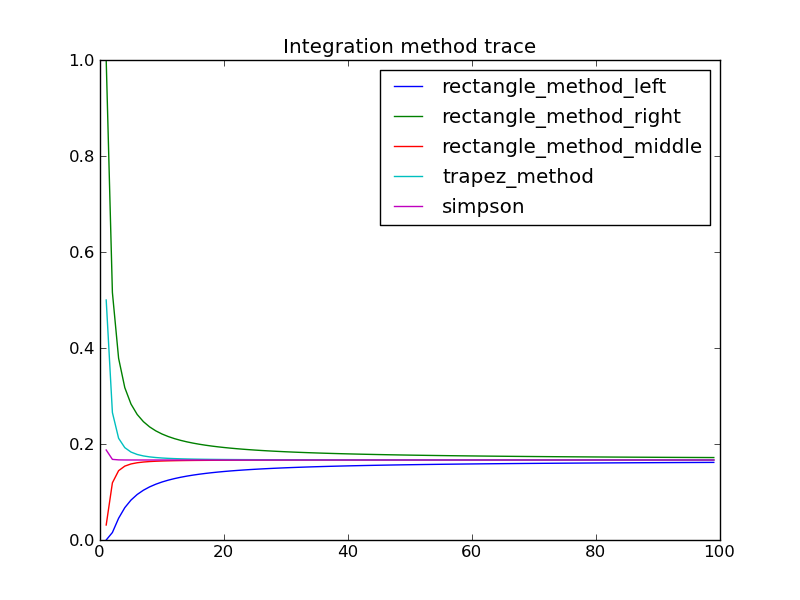
\includegraphics{../src/integration.png}
    \caption{power convergence comparison}
    \ref{comp}
\end{figure}

As we can see the Simpson method converges faster then the other ones to the same result.

\section{Computing the pressure map}
With the airfoil length it is possible to compute the pression of the air around the airfoil.
Anyway if we want to be able to compute this pression, we will have to model the air flow.

\subsection{Modeling the laminar air flow}
Even if the real air flow around an airfoil is not laminar, this model have been choose to make the computation easier.
The laminar air flow can be modeled by using the formula below, each one of the curves obtained represent the path followed by an air particule.

\subsection{Computing the pressure variation map}
The pressure on the airfoil will then depend of the length of each path. Indeed we assume that every air particule travel last the same time, the more length it will have to travel the more pression it will produce on the airfoil. 

\end{document}
